%appendix E
%HOLD QUEUE

\section{Process: Hold Queue}

\subsection{Overview}
\begin{figure}[ht]
    \centering
    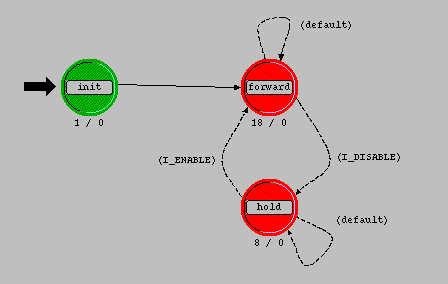
\includegraphics[width=.7\textwidth]{images/hold_queue}
    \caption{Hold queue process model}
    \label{fig:appendix-e}
\end{figure}

\subsection{Local variables}
\begin{figure}[ht]
    \centering
    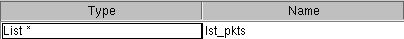
\includegraphics[width=.7\textwidth]{images/state_variable_hold_queue}
    \caption{State variables of hold queue process}
    \label{fig:appendix-e_sv}
\end{figure}

\subsection{Header Block}
%_____________________________________HEADER______________________________________
{\tiny
\begin{verbatim}
#define IC_DISABLE	54
#define IC_ENABLE	55
#define I_DISABLE	(op_intrpt_type() == OPC_INTRPT_REMOTE && op_intrpt_code() == IC_DISABLE)
#define I_ENABLE	(op_intrpt_type() == OPC_INTRPT_REMOTE && op_intrpt_code() == IC_ENABLE)

\end{verbatim}
}

\subsection{Function Block}
%______________________________FUNCTION__________________________________
{\tiny
\begin{verbatim}


\end{verbatim}
}
\subsection{init State: Enter Executives}
%______________________________________Init_____________________________________________________________
{\tiny
\begin{verbatim}
lst_pkts = op_prg_list_create (); 
\end{verbatim}
}

\subsection{forward State: Enter Executives}
%______________________________________forward_____________________________________________________________
{\tiny
\begin{verbatim}
Packet *pPkt;
int len;
len = op_prg_list_size(lst_pkts);

while(len > 0)
{
	printf("[HOLD] - Sending buffered pkt\n");
	op_pk_send(op_prg_list_remove (lst_pkts, OPC_LISTPOS_HEAD), 0);
	printf("\t[HOLD] - Done sending buffered pkt\n");
	len = op_prg_list_size(lst_pkts);	
}
pPkt = op_pk_get(0);
while(pPkt != OPC_NIL)
{
	op_pk_send(pPkt, 0);
	pPkt = op_pk_get(0);
}

\end{verbatim}
}

\subsection{hold State: Enter Executives}
%_____________________________________hold_____________________________________________________________
{\tiny
\begin{verbatim}
Packet *pPkt;
pPkt = op_pk_get(0);

while(pPkt != OPC_NIL)
{
	op_prg_list_insert(lst_pkts, pPkt, OPC_LISTPOS_TAIL);
	pPkt = op_pk_get(0);
}

\end{verbatim}
}